\large{
Di seguito, come anticipato nel capitolo precedente, sarà analizzata l'operazione di riduzione eseguibile mediante una interazione dell'utente con il sistema. Data la sua importanza si è scelto di trattarla in capitolo separato rispetto alle altre operazioni eseguibili. Per quanto riguarda i concetti introduttivi e le definizioni varie che saranno applicate in questo capitolo si rimanda al capitolo relativo allo stato dell'arte.
\section{metodo}
\begin{figure}[!htb]
	\begin{center}
		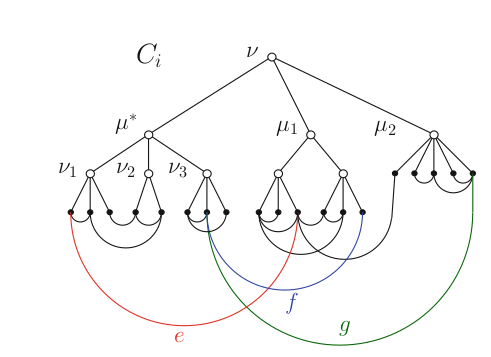
\includegraphics[width=0.8 \linewidth]{figure/preFlat}
	\end{center}
	\caption{$C_i$ con albero di inclusione $T$ omogeneo \label{fig:preFlat}}
\end{figure}
Ritornando a quanto visto nello stato dell'arte una istanza $C(G,T)$ di un c-graph, che nel nostro caso è rappresentata dall'oggetto \textit{clusteredGraph} di cui l'utente ne gestisce dati e visualizzazione, con n vertici e c cluster può essere ridotta in tempo $O(n+c)$ in una istanza equivalente $C_f(G_f,T_F)$ in cui T è omogeneo, la$r(T)$ definita come la radice dell'albero ha almeno due figli e $h(T)<=n-1$. \\
In altre parole l'obiettivo è quello di poter rappresentare un qualunque albero di inclusione con una profondità $d$ in un albero in cui la profondità massima è uguale a due, tutti i nodi interni sono cluster e tutte le foglie sono archi senza avere una perdita di informazioni intesa come numero di nodi o collegamenti tra di essi. La riduzione consiste in una sequenza di trasformazioni di $C$ = $C_0$ in $C_1$, $C_2$,. . . , $C_S(T) = C_f$, dove:
$$C_i = <G_i, T_i>$$
$$i = 0, 1,. . . , S(T)$$
in cui $C_i$ ha un albero di inclusione omogeneo $T_i$,ogni trasformazione richiede $O(n)$ tempo e $S(T)$ è definito come la dimenzione dell'albero di inclusione $T$, ovvero il numero di nodi superiori di $T$ diversi dalla radice.\\
Prendendo come mostrato in figura \figurename~\ref{fig:preFlat} un grafo clusterizzato nella sua rappresentazione "layered" è possibile vedere come esso rispetti le condizioni imposte in quanto l'albero di inclusione risulta omogeneo. È possibile dunque costruire $C_{i+1} = <G_{i+1},T_{i+1}>$ come segue ottenendo la rappresentazione mostrata nella figura \figurename~\ref{fig:postFlat}:\\
\begin{itemize}
	\item \textbf{$ G_{i+1} $} è ottenuto introducendo $\forall e=<u,v>$ di $\mu^*$, dove $\mu^*$ è un cluster ed $e$ è un arco inter-cluster, ovvero un arco si connessione tra i due nodi $u$ e $v$ appartenenti a cluster diversi, due nuovi vertici definiti $e_\chi$ ed $e_\varphi$ e sostituendo $e$ con un percorso $$(u, e_\chi)(e_\chi, e\varphi) (e_\varphi, v)$$
	\item \textbf{$T_{i+1}$} è ottenuto rimuovendo $\mu^*$, attaccando i suoi figli $v_1, v_2,. . . , v_h$ direttamente al cluster radice $v$ e aggiungendo ad esso due nuovi figli $\chi$ e $\varphi$, i quali conterranno tutti i vertici introdotti nella sostituzione di un arco inter-cluster di  $\mu^*$ con un sentiero.
\end{itemize}
\begin{figure}[!htb]
	\begin{center}
		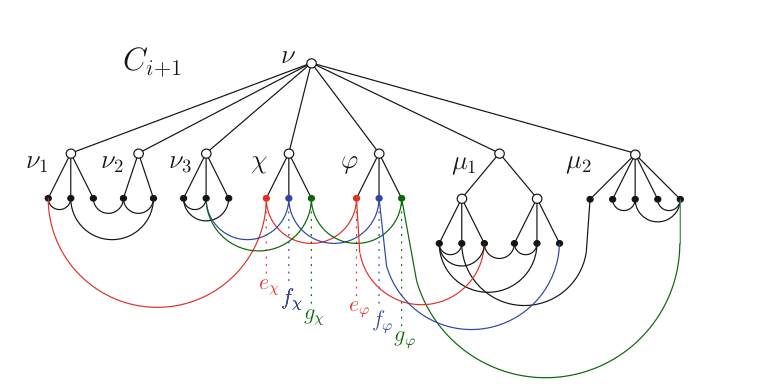
\includegraphics[width=1 \linewidth]{figure/postFlat}
	\end{center}
	\caption{$C_{i+1}$ ottenuto dopo parte del processo di riduzione \label{fig:postFlat}}
\end{figure}
Iterando la costruzione $\forall i$ si arriva ad avere un albero di inclusione $T$ di profondità $d=2$ in cui ogni cluster $c$ è un nodo interno dell'albero ed ogni foglia è rappresentata da un nodo dell'underlying graph, ovvero $T$ flat e nel grafo non si è persa conoscenza o connessione tra i nodi che risulteranno essere connessi comunque tra loro.
\begin{figure}[!htb]
	\begin{center}
		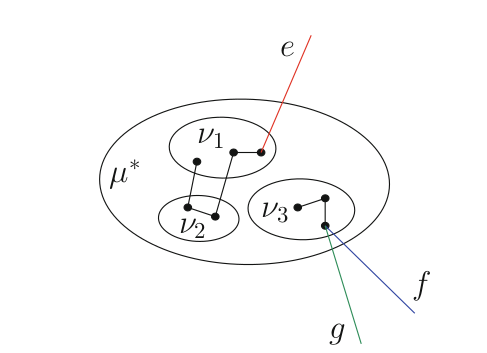
\includegraphics[width=1 \linewidth]{figure/dettaglioCluster}
	\end{center}
	\caption{Dettaglio del cluster $\mu^*$ con rappresentazione Spring-enbedding \label{fig:dettaglioCluster}}
\end{figure}
È inoltre possibile visualizzare la riduzione senza dover necessariamente utilizzare l'albero di inclusione. Partendo da una rappresentazione node-link con il metodo Spring-embedding del grafo cluterizzato ed in particolare soffermandosi solamente sul dettaglio del cluster $\mu^*$ di livello $l>2$ visualizzato in \figurename~\ref{fig:dettaglioCluster} è possibile eseguire una visualizzazione post-riduzione, seguendo i passi visti prima per la costruzione del grafo clusterizzato $C_{i+1} = <G_{i+1},T_{i+1}>$, con un modello Node-link. In questa rappresentazione  che è mostrata nella \figurename~\ref{fig:flatSpring} però i cluster aggiunti, che vanno a sostituire l'originale $\mu^*$, hanno una forma non più circolare ma ad anello. Questi cluster $\chi$ e $\varphi$ per permettere una maggiore copertura per quanto riguarda i possibili nodi $e_\chi$ ed $e_\varphi$ circonderanno i cluster che in precedenza appartenevano alla lista dei figli di $\mu^*$
\begin{figure}[!htb]
	\begin{center}
		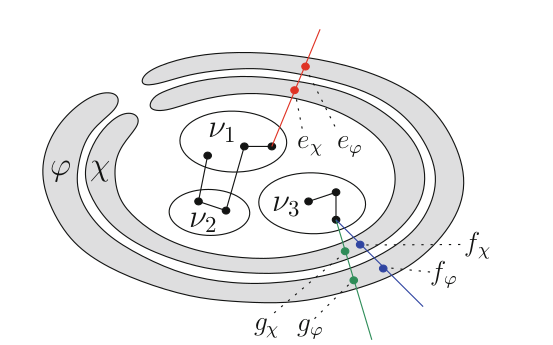
\includegraphics[width=1.1 \linewidth]{figure/flatSpring}
	\end{center}
	\caption{Cluster $\mu^*$ dopo la riduzione con rappresentazione semi Spring-enbedding \label{fig:flatSpring}}
\end{figure}
Per completezza si riportano le caratteristiche saltate in questa sezione fino ad ora che rappresentano ovvietà non specificate:
\begin{itemize}
	\item Se l'albero di inclusione $T_i$ è omogeneo, allora $T_{i + 1}$ è omogeneo, in quanto ogni nodo interno non avrà comunque nodi cluster e non al suo interno dopo la riduzione.
	\item $S(T{i+1}= S(T_i)-1$, ricordando che $S(T)$ è la dimenzione dell'albero $T$
	\item il grafo clusterizzato $C_f = C_{S(T)}$ è flat.
\end{itemize} 
Per concludere si può dunque denotare che 
\begin{center}
	$C_i(G_i , T_i )$ è un disegno planare \textbf{c-planar} di un grafo clusterizzato se e solo se anche $C_{i+1}(G_{i+1} , T_{i+1} )$ è un disegno planare 
\end{center}
$$C i (G i , T i ) is c-planar if and only if C i+1 (G i+1 , T i+1 ) is c-planar$$
\section{algoritmo}
%%citare titto
Definita e chiarita la riduzione polinomiale ideata dal professor Patrignani dell'università Roma Tre si passa ora all'operazione di trasformazione che l'utente, mediante una interazione su un bottone On/Off, potrà richiedere. Si è scelto di dare la possibilità all'utente di poter tornare alla visualizzazione precedente la trasformazione dei dati di modo da poter continuare la sessione e vedere potenziali differenze tra grafi clusterizzati e le loro riduzioni.
\begin{figure}[!htb]
	\begin{center}
		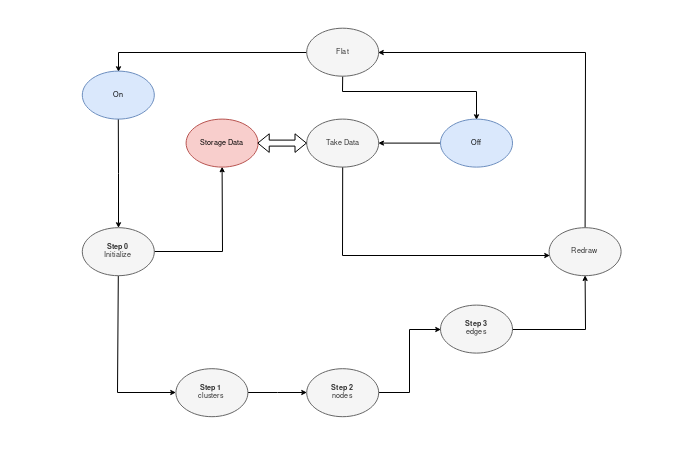
\includegraphics[width=1.1 \linewidth]{figure/flatAlg}
	\end{center}
	\caption{Struttura semplificata dell'algoritmo di flattizzazione \label{fig:flatAlg}}
\end{figure}
Lavorando nella visualizzazione a grafo, ovvero la \textit{graph-view}, ed avendo ultimato una prima analisi l'utente chiederà al sistema di eseguire la riduzione. Il sistema risponderà eseguendo l'algoritmo mostrato schematicamente nella \figurename~\ref{fig:flatAlg} e riportato di seguito in maniera semplificata. Alla base, l'algoritmo di riduzione in grafo clusterizzato flat è composto dai seguenti step:
\begin{itemize}
	\item \textbf{Step 0} Inizializzazione;
	\item \textbf{Step 1} Creazione cluster sostitutivi;
	\item \textbf{Step 2} Creazione dei nodi aggiuntivi;
	\item \textbf{Step 3} Sostituzione archi con percorsi;
	\item \textbf{Step 4} visualizzazione della classe \textit{clusteredGraph} ora resa Flat.
\end{itemize}
Nella fase di inizializzazione il sistema prima di eseguire qualunque cambiamento sugli oggetti creati e/o importati dall'utente provveder ad eseguire una copia di questi dati per poter eseguire operazioni di ritorno ai valori pre-riduzione e continuarne la modifica. Successivamente vengono creati delle liste contenenti solo ed esclusivamente gli oggetti del grafo su cui eseguire la riduzione, quali nodi con archi uscenti e cluster con livello $l>2$.\\
Superata la fase di inizializzazione si passa alla trasformazione dei dati. Nello step 1 $\forall$cluster $\mu_i, \forall i=0,...,l.length$ con l uguale alla lista dei cluster da cambiare inizializzata in precendenza, questo viene eliminato ed al suo posto vengono inseriti due oggetti cluster che possiederanno come attributo label l'etichetta del cluster $\mu_i$ a cui sarà unita la lettera $X$ o $Y$. 
Creati i cluster si passa poi al secondo step ovvero all'aggiunta dei nodi aggiuntivi. In particolare $\forall$nodo $n_i, \forall i=0,...,nodes.length$ con nodes uguale alla lista dei nodi da cambiare inizializzata,si creeranno, $\forall$ arco esterno del loro \textit{rotationScheme} $e_i$ due nodi $n_iX$ ed $n_iY$ rispetivamente interni ai cluster creati prima che hanno sostituito quello in cui il nodo risiedeva.
Nel terzo step creati cluster e nodi si puù passare alla rimozione degli archi intercluster appartenenti alla lista degli archi da cambiare e alla creazione del percorso $(source, e_\chi)(e_\chi, e\varphi) (e_\varphi, target)$
Terminate le trasformazioni il sistema concluderà con una operazione di visualizzazione della struttura dati mediante la rappresentazione riportata nella Tree-view come mostrato nella \figurename~\ref{fig:esempioTreeRidotto}.
In qualunque momento l'utente potrà tornare alla visualizzazione del grafo non ancora ridotto e continuare il lavoro svolto.
\begin{figure}[!htb]
	\begin{center}
		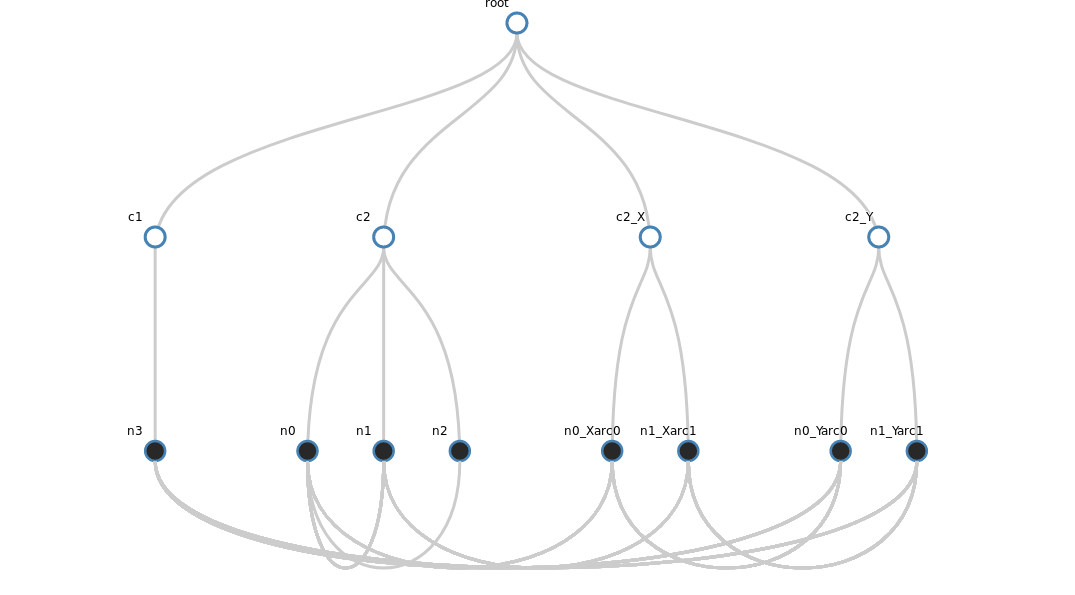
\includegraphics[width=1 \linewidth]{figure/esempioTreeRidotto}
	\end{center}
	\caption{Esempio della riduzione di un grafo clusterizzato nella Tree-View \label{fig:esempioTreeRidotto}}
\end{figure}
Esempi reali di utilizzo di questa riduzione saranno visti nel dettaglio nel capitolo successivo in cui verranno utilizzate la maggior parte delle interazione ed operazioni dell'utente in cui saranno eseguite simulazioni reali di utilizzo e di test non solo sulle connessioni tra gli oggetti che compongono il grafo clusterizzato ma anche sulla loro visualizzazione. Il sistema inoltre non pone alcun messaggio di errore nel caso in cui l'utente decida di effettuare di riduzione del grafo clusterizzato in quanto non previsto che vengano eseguiti controlli su grafi erroneamente disegnati. Questo porta sicuramente a errori iniziali da parte dell'utente nell'approccio con il sistema ma dona anche la possibilità di eseguire qualunque operazione e grafo si decida di realizzare lasciando pieno controllo umano.
}
